% This paper is written for CHASE 2013 and features the concept and
% creation of "Impact" the awareness tool.

\documentclass[conference]{IEEEtran}

\usepackage{graphicx}
\usepackage{amsmath}

\hyphenation{op-tical net-works semi-conduc-tor}

\begin{document}

%Paper title
\title{Supporting Awareness of Indirect Conflicts with Impact}

%Author block
\author{\IEEEauthorblockN{Jordan Ell}
\IEEEauthorblockA{University of Victoria\\
Victoria, British Columbia \\ jell@uvic.ca}
\and
\IEEEauthorblockN{Daniela Damian}
\IEEEauthorblockA{University of Victoria\\
Victoria, British Columbia \\ danielad@cs.uvic.ca}}

\maketitle

% Paper abstract
\begin{abstract}
Awareness has been largely studied in the field of CSCW research within
software engineering. Many tools and techniques have been proposed and built
in order to provide software developers and stakeholders with a greater
sense of workspace and task awareness within their software projects. These
techniques and tools have been largely focused on detecting \textit{direct} 
conflicts which arise over a project's life time or have created 
an exploratory ground for stakeholders to use as a means of resolving self
discovered direct or indirect conflicts. However, detecting 
and providing pertinent information regarding \textit{indirect} conflicts has been
largely ignored partially due to their inherently larger
complexity than direct conflicts. Indirect conflicts arise when changes
in one software artifact affect another. In this paper, we present
\textit{Impact}, a new task awareness tool directly aimed at both detecting
and presenting indirect conflicts which arise inside of a software project.
\textit{Impact} represents a first step towards the design and implementation
of awareness tools that specifically address indirect conflicts in software
projects. To describe \textit{Impact}, we introduce previous indirect 
conflict awareness attempts, our design 
and implementation, as well as \textit{Impact's} potential through
two evaluation studies. 
\end{abstract}


\section{Introduction}
Awareness is characterized as "an understanding of the activities of others
which provides a context for one's own activities"~\cite{Dourish:1992:ACS}.
The study of awareness and its tools has become an important topic of
research in software engineering especially with the new importance of
distributed work and collaboration. Awareness is generally associated with
both technical and social dependencies that are created and evolve over
a software project's life time. The study of these dependencies has become
the primary focus of most awareness related research. Task awareness has
become the most prevalent field of awareness research to understand 
how developers cope with these technical and social dependencies.

Tools have been created to attempt to solve task awareness related issues
with some success~\cite{Xiang:2008:ERT, Biehl:2007:FVD, Sarma:2009:TIV, Khurana:2009:PFC}. However, these tools have been designed 
to solve task awareness related issues at the direct conflict level. 
Examples of direct conflict awareness include knowing when two or more 
developers are  editing same artifact, finding expert knowledge of a
particular file, and knowing which developers are working on which files.
Meanwhile, task awareness related issues at the indirect conflict level
continue to be an issue which is largely unsolved by most coordination
mechanisms. Examples of indirect conflict awareness
include having one's own code effected by another developer's source
code change or finding out who might be indirectly effected by one's
own code change. Previous interviews and surveys conducted with software developers have 
shown a pattern that developers of a software project view indirect conflict 
awareness  as a high priority issue in their development~\cite{Damian:2007:GSE, 
Halverson:2006:DTV, Begel:2010:CDE, Schroter:2012:TTF}.

Indirect conflicts arising in source code are inherently
difficult to resolve as most of the time, source code analysis must
be performed in order to find relationships between technical objects
which are harmed by changes.
While some awareness tools have been created with these indirect conflicts
primarily in mind~\cite{Begel:2010:CDE, Trainer:2005:BGT}, most have only 
created an exploratory environment which is used by developers to
solve conflicts which may arise. These tools were not designed to detect
indirect conflicts that arise and alert developers to their presence 
inside the software system. Sarma et al.~\cite{Sarma:2007:TSA} has started to work directly
on solving indirect conflicts, however, these products are not designed to handle
internal structures of technical objects.

In this paper, we report on our research into supporting indirect conflicts
and present the design, implementation, and evaluation of the tool \textit{Impact},
a web based tool that aims at detecting indirect conflicts among developers
and notifying the appropriate members involved in these conflicts.
By leveraging technical relationships inherent of 
software projects with method call graphs~\cite{Lakhotia:1993:CCM}
as well as detecting changes
to these technical relationship through software configuration management
(SCM) systems, \textit{Impact} is able to detect indirect conflicts as well as
alert developers involved in such conflicts in task awareness. While this paper
outlines \textit{Impact's} specific implementation, its design is rather
generic and can be implemented in similar indirect conflict awareness tools.
\textit{Impact} represents a first step towards the design and implementation
of awareness tools which address indirect conflicts in software development.

The rest of this paper is organized as follows. First, we begin by discussing
similar indirect conflict awareness tools which have partially solved the
issues presented by this paper and how their designs can be applied to 
\textit{Impact}. In the following section we describe a generic design and implementation
of \textit{Impact} as an awareness tool. We then discuss a preliminary evaluation of
\textit{Impact} followed by conclusions and future work.


\section{Related Work}
Although there is an abundance of awareness tools developed in research
today, only a handful have made an attempt to examine indirect conflicts.
Here, we will outline three of the forefront projects in indirect conflicts
and how these projects have influenced the decision making process in
the design and implementation of \textit{Impact}.

We first start with both Codebook~\cite{Begel:2010:CDE} and 
Ariadne~\cite{Trainer:2005:BGT}. These projects produce an exploratory
environment for developers to handle indirect conflicts. Exploratory
pertains to the ability to solve self determined conflicts, meaning that
once a developer discovers a conflict, they can use the tool as a type of
lookup table to solve their issue. Codebook is a type of social developer
network that relates developers to source code, issue repositories and
other social media while Ariadne only looks at source code for developer
to source code association. Through Codebook, developers become
owners of source code artifacts. Both projects also use program 
dependency graphs~\cite{Horwitz:1992:UPD}
in order to relate technical artifacts to each other. These projects make 
use of method call graphs in order to 
determine which methods invoke others which forms the basis for 
linking source code artifacts creating a directed graph. While these 
projects can be great tools 
for solving indirect conflicts which may arise, by querying such directed
graphs to view impacts of conflict creating code, they lack the ability to
detect conflicts on their own.

A serious attempt at both detecting and informing developers of
indirect conflicts is the tool Palantir~\cite{Sarma:2007:TSA}. Palantir
monitors developers activities in files with regards to class signatures.
Once a developer changes the signature of a class, such as by modifying changes
in name, parameters, or return values of public methods, any workspace
of other developers which are using that class will be notified. Palantir utilizes
a push-based event model~\cite{Fitzpatrick:2002:SPA} which seems to be
a favored collection system among awareness tools. Sarma et al.
~\cite{Sarma:2007:TSA} also
developed a generic design for future indirect conflict awareness tools. 
However, Palantir falls short in its collection and distribution
mechanisms. First, Palantir only considers "outside" appearance of technical
objects, being their return types, parameters, etc. Secondly, Palantir 
only delivers
detected conflicts to developers who are presently viewing or editing
the indirect object while other developers who have used the modified 
class previously are not notified.

\textit{Impact} is designed to address these limitations by extending this work in
two directions: (1) the detection of indirect conflicts at an internal level
of technical objects as opposed from object signatures, and (2) the dissemination of
awareness information to all appropriate developers regardless of their current
workspace activities. \textit{Impact} is also designed around the successes these
projects have had in the past with directed graphs as 
well as elements of collection, ownership, and distribution functionality.


\section{Impact}
This section will proceed to give an outlined detail of \textit{Impact} in both its
design and implementation. The design of \textit{Impact} was created to be
a generic construct which can be applied to other indirect conflict 
awareness tools while the implementation is specific to the technical
goals of \textit{Impact}.

\subsection{Design}
Compared to tool design for direct conflicts, the major concern of 
indirect conflict tools is to relate technical objects to one another
with a ``uses'' relationship. To say that object 1 uses object 2 is to infer
a technical relationship between the two objects which can be used
in part to detect indirect conflict that arise from modifying object
2. This kind of relationship is modeled based on directed graphs ~\cite{Horwitz:1992:UPD}. 
Each technical object is represented by node while each ``uses''
relationship is represented by a directed edge. This representation
is used to indicate all indirect relationships within a software project.

\begin{figure}[t!]
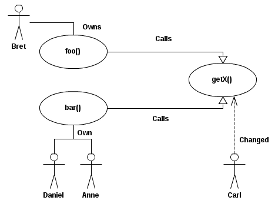
\includegraphics[width=\columnwidth]{images/CallGraph}
\caption{Technical object directed graph with ownership\label{fig:graph}}
\end{figure}

While technical object relationships form the basis of indirect conflicts,
communication between developers is the ultimate goal of resolving such conflicts.
This being the case, developer ownership must be placed on the 
identified technical objects. With this ownership, we now infer
relationships among developers based on their technical objects
``uses'' relationship. Developer A, who owns object 1, which uses 
object 2 owned by developer B, may be notified by a change to
object 2's internal workings. Most, if not all, ownership information
of technical objects can be extracted from a project's source code
repository (CVS, Git, SVN, etc.).

Finally, the indirect conflict tool must be able to detect changes
to the technical objects defined above and notify the appropriate owners
to the conflict. 
Two approaches have been 
proposed for change gathering techniques: real time and commit 
time~\cite{Fitzpatrick:2002:SPA}.
We propose the use of commit time
information gathering as it avoids the issue of developers 
overwriting previous work or deleting modifications which would 
produce information for changes that no longer exist. However, the
trade off is that indirect conflicts must be committed before detected,
which results in conflicts being apart of the system before being able
to be dealt with as opposed to catching conflicts before they happen.
At commit time, the tool must parse changed source code in relation
to technical artifacts in the created directed graph detailed above.
Where \textit{Impact's} design differs from that of Palantir's is that
the object's entire body (method definition and internal body) is 
parsed at commit time to detect changes anywhere in the technical object.
Once technical objects are found to be changed, appropriate owners
of objects which use the changed object should be notified.
In Figure~\ref{fig:graph}, Carl changes method (technical object) 1,
which effects methods 2 and 3 resulting in the alerting of
developers Bret, Daniel, and Anne.

With this three step design: (i) creating directed graphs of technical
objects, (ii) assigning ownership to those technical objects, and (iii)
detecting changes within commit time and the notification of conflict information
to appropriate owners, we believe a wide variety of
indirect conflict awareness tools can be created or extended. The
implementation of \textit{Impact} described in the following section follows these
three design guidelines.

\subsection{Implementation}
For \textit{Impact's} implementation, we decided to focus on methods as our
selected technical objects to infer a directed graph from. The ``uses'' 
relationship described above for methods is method invocation.
Thus, in our constructed directed graph, methods represent nodes
and method invocations represent our directed edges. In order to 
construct this directed graph, abstract syntax trees (ASTs) are 
constructed from source files in the project. The ASTs allow us
to construct method call graphs from which the directed 
graphs can be constructed.

Once the directed graph is constructed, we must now assign
ownership to our technical objects (methods) as per our design.
To do this, we simply query the source code repository. In our case
we used Git as the source code repository, so the command \textit{git blame}
is used for querying ownership information. (Most source code 
repositories have similar commands and functionality.) This command 
returns the source code authors per linee which can is used to assign
ownership to methods. If a method has 10 lines and developer A
has written 3 while developer B has written 7, then ownership is
assigned 30\% and 70\% respectively.

To detect changes to our technical objects (methods), we simply 
use a commit's \textit{diff} which is a representation of all changes
made inside a commit. We can use the lines changed in the \textit{diff} to 
find methods that have been changed. This gives cause of potential
indirect conflicts. We now find all methods in our directed graphs
which invoke these changed methods. These are the final indirect
conflicts.

Once the indirect conflicts have been found, we use the
ownership information of our technical objects to send notifications to
those developers involved in the indirect conflict. All owners
of methods which invoke those that have been changed are alerted
to the newly changed method. This can been seen in
Figure~\ref{fig:impact}, the user interface of \textit{Impact}. Here, in an RSS type
feed, the changing developer, time of change, changed method,
invoking methods, and commit message are all displayed. This 
list is auto updating as new commits are pushed to the central
git repository. The information provided also comes with a simple
weight of the percent changed of changed method multiplied by 
ownership of the invoking method. This allows developers to filter
through high and low changes affecting their own source code.
Developers are now able to be alerted of detected indirect
conflicts and solve them by communicating the developer
who authored the change.

\begin{figure}[t!]
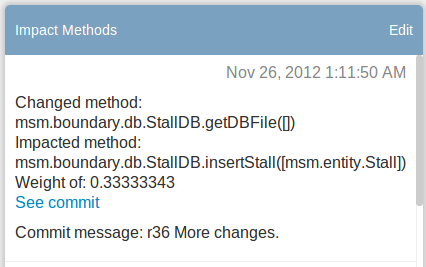
\includegraphics[width=\columnwidth]{images/ImpactDemo}
\caption{\textit{Impact's} RSS type information feed.\label{fig:impact}}
\end{figure}


\section{Evaluation}
To fully evaluate both the generic design of detecting and resolving
indirect conflicts as well as \textit{Impact}, extensive testing and evaluation
must be performed. However, we feel that a simple evaluation is
first needed to assess the foundation of \textit{Impact}'s design and claims
about indirect conflicts at the method level.

We performed a user case study where we gave \textit{Impact} to 
two small development teams composed of three developers. Each team was
free to use \textit{Impact} at their leisure during their development process,
after which interviews were conducted with lead developers from 
each development team. The interviews were conducted after each
team had used \textit{Impact} for three weeks.

We asked lead developers to address two main concerns: do indirect
conflicts pose a threat
at the method level (e.g. method 1 has a bug because it invokes method
2 which has has its implementation changed recently), 
and did \textit{Impact} help raise
awareness and promote quicker conflict resolution for indirect
conflicts. Our two interviews largely supported our expectation of
indirect conflicts posing a serious threat to developers, especially
in medium to large teams or projects as opposed to the small
teams which they were apart of. It was also pointed
out that method use can be a particularly large area for indirect
conflicts to arise. However, it was noted that
any technical object which is used as an interface to some data
construct or methodology, database access for instance, can be 
a large potential issue for indirect conflicts.  Interview response to
\textit{Impact} was also largely positive, as interviewees stated that \textit{Impact}
helped raise awareness among their teams with what other developers
are doing as well as the influence it has on their own work. However,
\textit{Impact} was shown to have information overload. It was suggested
that while all method changes were being detected,
not all are notification worthy. One developer suggested to only notify
developers to indirect conflicts if the internal structure of a method
changes due to modification to input parameters or output parameters.
In other words, the boundaries of the technical objects (changing
how a parameter is used inside the method, modifying the return
result inside the method) seem to be more of interest than other 
internal workings. More complex inner workings of methods were also noted 
to be of interest to developers
such as cyclomatic complexity, or time and space requirements.

These two studies have shown that our design and approach to
detecting and alerting developers to indirect conflicts appear
to be on the correct path. \textit{Impact} as a tool has laid the foundations
for future work in detecting indirect conflicts as well as notifying
developers, although more thought must be given as to 
what constitutes a meaningful change inside our selected 
technical objects to avoid issues of information overload.

\section{Next Steps in Research of Indirect Conflicts}
While \textit{Impact} has laid the foundations for awareness tool construction
aimed at resolving indirect conflicts, it has also raised questions 
in regards to levels of granularity in notification of indirect conflicts and the
implied trade off between notifications and information overload. To address
these problems, we plan to find industry expert opinion through interviews
and surveys with experienced developers. From these interactions, we plan to
answer some of the questions presented in this paper such as which technical
objects concern developers with indirect conflicts, and what types of changes
to these objects are cause for notification. We are also planning, through these
expert opinions, to further the 
need for indirect conflict awareness tools by establishing that indirect
conflicts are real world problems with harmful consequences. 
Further more, we plan to bring these opinions back to the realm of 
\textit{Impact}, in combination with other academic works on balancing
between notifications and information overload~\cite{Wang:2007}, to
continue our development
on this tool to further its life both as a research tool and a possible
industry application. 

\section{Conclusion and Future Work}
In this paper, we have presented the issues that arise from indirect 
conflicts in present awareness tools. We have proposed a generic 
design for the future development of awareness tools in regards to
handling indirect conflicts. We have presented a prototype 
awareness tool, \textit{Impact}, which was designed around our generic 
technical object approach. \textit{Impact} was evaluated on a small scale, showing
its future potential as well as highlighting its current weaknesses. 
Our preliminary evaluation has given us concrete insights into 
understanding awareness tools that specifically address indirect conflicts and has
strengthened the need for further research towards notification and information
overload (what makes a change notification
worthy), which has become the goal of our next step.


\bibliographystyle{IEEEtran}
\bibliography{paper}

%End of paper
\end{document}